\chapter{The Demo}

This section aims to explain the overall architecture and choices made for the demo, specific solutions for synchronization will be presented in the next chapter. 

All code is available at github: https://github.com/Rymdsnigel/thesis-demo

\section{Running the programs}
The demo program is written in python 2.7.2. It requires pygame 1.9.1, simplejson 2.1.6, docopt 0.6.1 and gevent 0.13.0. 

% How its started
% How to interact with the server

\section{Overall architecture}
The demo program consists of a server that continously accept connecting clients. 

\begin{figure}[h!]
\centering
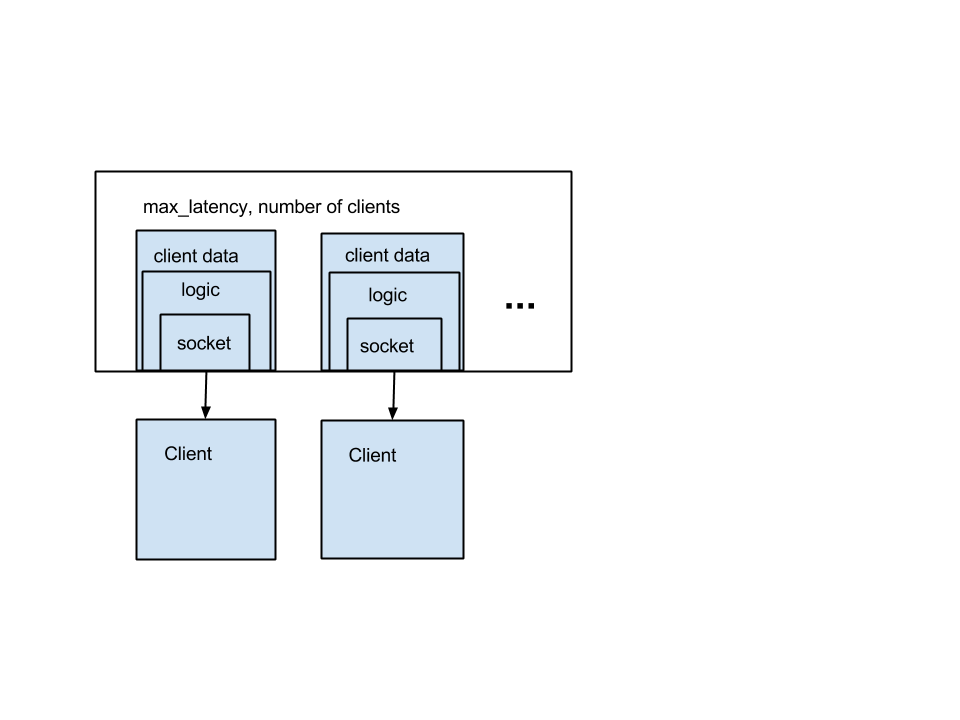
\includegraphics[width=1.0\textwidth]{figures/arch.png}
\caption{Overall architecture of the system.}
\end{figure}

\subsection{Why the Client-Server approach?}
Because there was a need to both generate and distribute specific events the client-server approach were chosen, rather than choosing a master among the clients, which might have been a more flexible choice if the generation of events had not been in the specification. The downside of this is that if the server should crash, the clients will loose their connection, the connection will not be reestablished by restarting the server.

\section{Design choises}

\section{Communication}

\subsection{Protocols}
The choice of TCP-sockets as opposed to UDP-sockets was made at an early stage of development. Although UDP is typically the ideal choice for time critical applications, customizing the needed control mechanisms would be outside the scope of this thesis. 

The choice of TCP presented proved to be problematic when it was discovered that TCP:s message buffering, using Nagels algoritm, generated a general delay in messaging, a delay of 20 ms both from the server as from the clients. This was discovered by measuring the delays of the application over localhost, where network delays should be close to 0. This issue also resulted in that more than one json object could be put on the queue of recieved events, which lead to a json-parsing error when trying to load the objects. These errors and the buffer delays were removed by disabling Nagels algorithm\footnote{\url{http://stackoverflow.com/questions/8617809/unstable-tcp-receive-times}} by setting the nodelay flag on the socket.

%source nagels algoritm

\begin{figure}[h!]
\centering
\texttt{self.s.setsockopt(socket.IPPROTO\_TCP, socket.TCP\_NODELAY, 1)}
\caption{Setting the nodelay flag on the socket}
\end{figure}

\subsection{Sockets}
The demo server communicates with the clients via gevent sockets since the sockets need to be threaded in order to not block the other processes. 

% ref to section about greenlets.
% explaining gevent sockets as opposed to regular sockets. 

\subsection{Replacing the networklayer}
Functional cohesion has been strived for, in order to make the part of the code pertaining to transport easily replaced by for example an implementation using UDP or implementation of a ready solution such as redis. Though this has not been entirely accomplished %in which ways is it not.






\subsection{Threading}
\label{sec:threading}

Both the server and the client has to achieve concurrency. This is achieved by letting both the TransportServers and the TransportClients inherit from gevent Greenlets %ref. 
Greenlets are in fact pseudothreads %ref
that share the same OS-thread so to release the control the threads must sleep on time critical operations to not block all other threads. 


\subsection{Messaging}
The server and clients sends and recieves json, the json is created using simplejson-library functions (dumps() and loads()), creating json from dicts. The functions for generating the dicts that will be the messages are specified in event.py. 

The choice of json for messaging, instead of using pickle or cpickle to read and write messages was made due to jsons speed of reading and writing \footnote{\url{http://kovshenin.com/2010/pickle-vs-json-which-is-faster/}, Kovshenin} and to support future flexibility in language since pickle and cpickle is python-specific. 

\subsection{Pygame}

Pygame, which is built on SDL(ref:http://www.pygame.org/wiki/about) was choosen for graphics due to its simplicity to work with. 



